\documentclass{article}
\usepackage{../math_template}

\title{STEP Support Programme --- Assignment 1}
\author{Jonathan Kasongo}

\begin{document}
\maketitle

We will only write up problems 3 and 4, since the others are trivial.

\begin{problem}{Problem 3}
In this question \(a\) and \(b\) are distinct, non-zero real numbers, and \(c\) is a real number.

\begin{enumerate}
    \item[(i)] Show that, if \(a\) and \(b\) are either both positive or both negative, then the equation
    \[
    \frac{x}{x - a} + \frac{x}{x - b} = 1
    \]
    has two distinct real solutions.

    \item[(ii)] Show that, if \(c \neq 1\), the equation
    \[
    \frac{x}{x - a} + \frac{x}{x - b} = 1 + c
    \]
    has exactly one real solution if
    \[
    c^2 = - \frac{4ab}{(a - b)^2}.
    \]
    Show that this condition can be written
    \[
    c^2 = 1 - \left( \frac{a + b}{a - b} \right)^2
    \]
    and deduce that it can only hold if \(0 < c^2 \leq 1\).
\end{enumerate}
\end{problem}

\begin{solution}{Solution to Problem 3}
For part (i), we have $2x^2 - (a+b)x = x^2 - (a+b)x + ab$ and so
$x^2 = ab$. If $a$ and $b$ have the same parity then $ab > 0$ (since $a,b$
are non-zero) and so $x^2 = ab$ will have 2 distinct real solutions, namely
$\sqrt{ab}$ and $-\sqrt{ab}$.\\

In part (ii) we get $2x^2 - (a+b)x = (1+c)x^2 - (a+b)x - c(a+b)x + ab +
abc$ and so $(c-1)x^2 - c(a+b)x + ab(c+1) = 0$. To have exactly one real
solution the discriminant must be 0 so, $\left[ c(a+b) \right]^2 =
4ab(c-1)(c+1)$. Now observe that,

\[
\begin{aligned}
c^2 &= \frac{4(c^2 - 1)ab}{(a+b)^2} \\
&= \frac{4c^2}{(a+b)^2} - \frac{4ab}{(a+b)^2} \\
c^2 \left(1 - \frac{4ab}{(a+b)^2}\right) &= - \frac{4ab}{(a+b)^2}\\
c^2 \frac{(a-b)^2}{(a+b)^2} &= - \frac{4ab}{(a+b)^2}
\end{aligned}
\]

and so we readily derive $c^2 = -\frac{4ab}{(a-b)^2}$, as desired. To do
the next part we can work backwards, we have

\[
\begin{aligned}
c^2 &= 1 - \left( \frac{a+b}{a-b} \right)^2 \iff \\
&= \left(1 - \frac{a+b}{a-b}\right)\left(1 + \frac{a+b}{a-b}\right) \iff \\
&= \left( -\frac{2b}{a-b} \right) \left( \frac{2a}{a-b} \right) \iff \\
&= -\frac{4ab}{(a-b)^2}\\
\end{aligned}
\]

but that is obviously true as we just showed that before.
Now finally to show that inequality, we know that for any real number
$x$, we have $x^2 \geq 0$ and so $c^2 \geq 0$. But $c^2 \neq 0$ since if
$c^2 = -\frac{4ab}{(a-b)^2} = 0$ then one of $a,b$ is 0, but this is
impossible (\textit{In this question \(a\) and \(b\) are distinct,
non-zero real numbers...}). Thus we have established $c^2 > 0$. To show
that $c^2 \leq 1$, note that $\left( \frac{a+b}{a-b} \right)^2 \geq 0$ and
so $c^2 = 1 - \left( \frac{a+b}{a-b} \right)^2 \leq 1$, as desired.
\end{solution}
\vspace{0.2cm}
\begin{problem}{Problem 4}
The diagram shows a circle $C$ with centre $O$, and a rod $AB$ the ends of which can slide round
the circle $C$ (so that $AB$ is a chord of $C$). The radius of the circle is $R$ and the length of the
rod is $2a$.
As the rod slides round $C$ the point $P$, which is a fixed distance $b$ from the centre of the rod,
traces out a circle with centre $O$ of radius $r$.\\

Show that the area between the 2 circles is $\pi (a^2 - b^2)$.
\end{problem}

\begin{solution}{Solution to Problem 4}
Observe the following diagram

\begin{center}
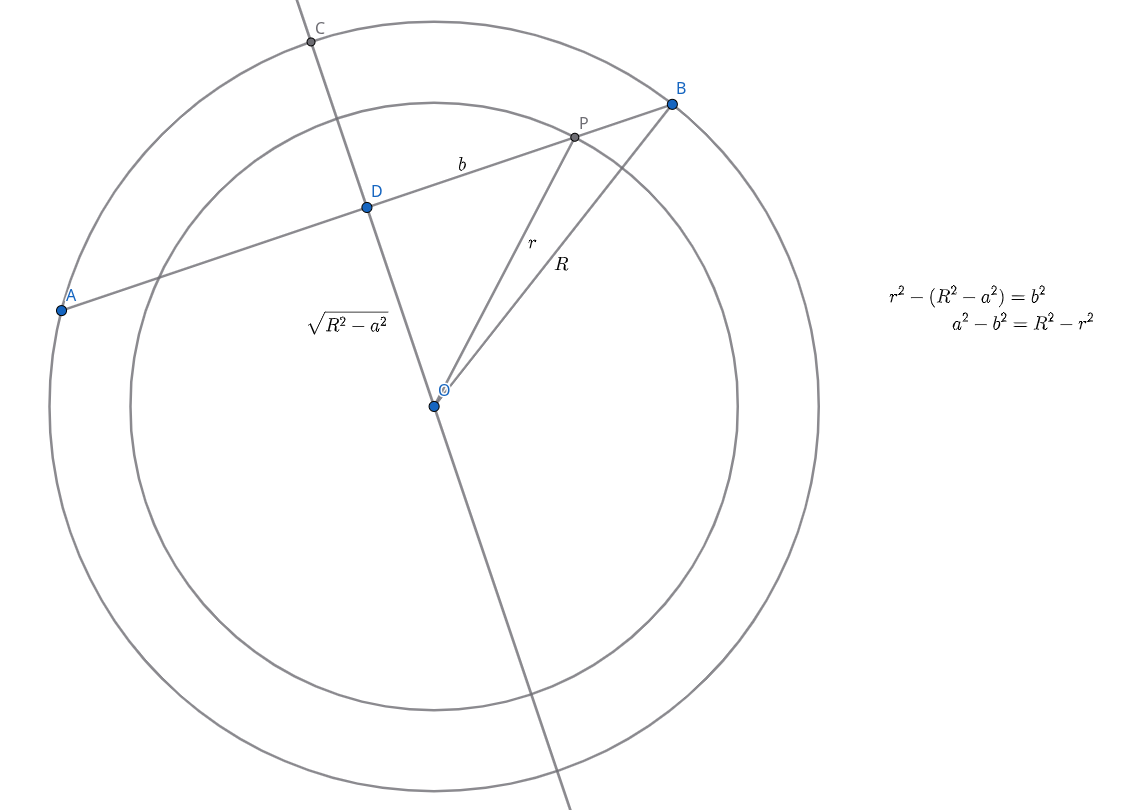
\includegraphics[scale=0.5]{STEP_MODULE_1_P4.png}
\end{center}

The area we are looking for is $\pi \left(R^2 - r^2\right) =
\pi \left(a^2 - b^2\right)$ as desired.
\end{solution}

\end{document}
